\documentclass{article}

\usepackage{tikz, multirow, multicol, pgfplots, booktabs}
\usetikzlibrary{calc}

\tikzset{
% Two node styles for game trees: solid and hollow
solid node/.style={circle,draw,inner sep=1.5,fill=black},
hollow node/.style={circle,draw,inner sep=1.5}
}

\begin{document}

		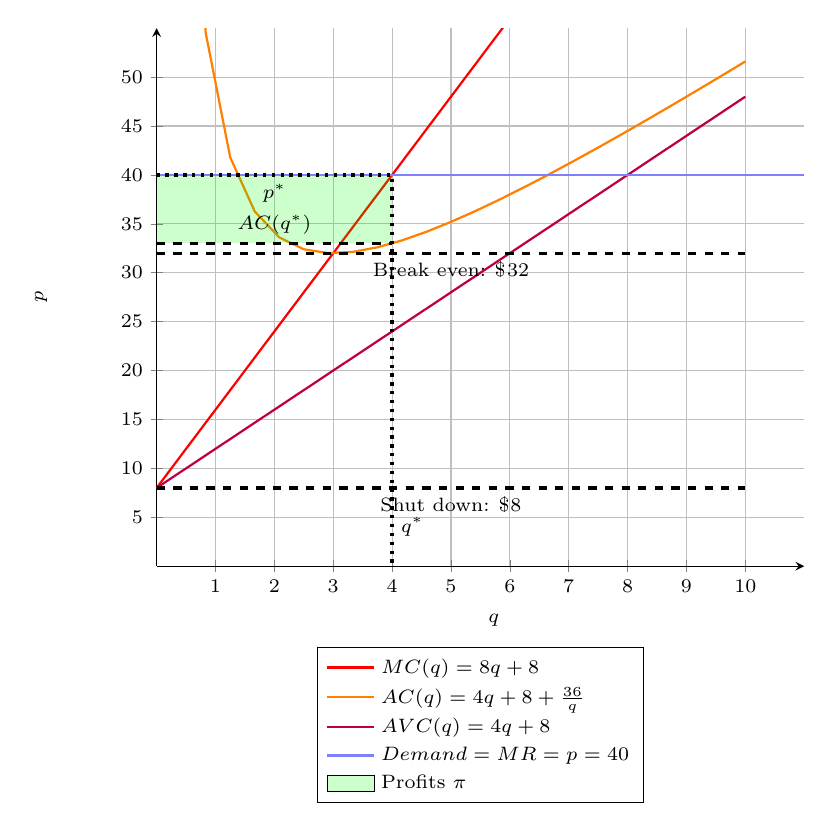
\begin{tikzpicture}\scriptsize 
	\begin{axis}[scale=1.2,
		xlabel=$q$,
		ylabel=$p$,
		grid=major,
		legend style={at={(0.5,-0.15)},anchor=north},
		legend cell align=left,
		axis lines=center,
		xtick={0,1,...,10},
		ytick={0,5,...,50},
		ymax=50,
		ymin=0,
		xmin=0,
		xmax=10,
		enlarge x limits={rel=0.1, upper},
		enlarge y limits={rel=0.1, upper},
		every axis y label/.style={at={(axis description cs:-0.2,0.5)},rotate=90,anchor=north},
		every axis x label/.style={at={(axis description cs:0.5,-0.1)},anchor=west},
		]
		\addplot[thick, domain=0:10,red, samples=20]{8*x+8};
		\addlegendentry{$MC(q)=8q+8$}
		\addplot[thick, domain=0:10,orange]{4*x+8+36/x};
		\addlegendentry{$AC(q)=4q+8+\frac{36}{q}$}
		\addplot[thick, domain=0:10,purple]{4*x+8};
		\addlegendentry{$AVC(q)=4q+8$}
				\addplot[thick, domain=0:11,blue!50]{40};
		\addlegendentry{$Demand=MR=p=40$}
		\addplot[fill=green, fill opacity = 0.2, draw = none,area legend] coordinates {(0,33) (0,40) (4,40) (4,33)};
        \addlegendentry{Profits $\pi$}; 
        \draw[dashed, very thick] (axis cs:0,33)--node[above]{$AC(q^*)$}(axis cs:4,33);
		\draw[dashed, very thick, black] (axis cs:0,8)--node[below]{Shut down: \$8}(axis cs:10,8);
	\draw[dashed, very thick, black] (axis cs:0,32)--node[below]{Break even: \$32}(axis cs:10,32);
	\draw[dotted, very thick, black] (axis cs:0,40)--node[below]{$p^*$}(axis cs:4,40)--(axis cs:4,0)node[above=.5cm, right]{$q^*$};
	\end{axis}
	\end{tikzpicture}

\end{document}